\documentclass{article}
\usepackage[margin=1in]{geometry}
\usepackage{graphicx}
\usepackage{url}
\usepackage{titlesec}
\usepackage{pifont}
\newcommand{\cmark}{\ding{51}}
\newcommand{\xmark}{\ding{55}}

\usepackage[pdfauthor={Arin Upadhyay}, pdftitle={EFPIX: A zero-trust encrypted flood protocol}, pdfkeywords={encryption, flooding, anonymity, zero-trust, protocol, decentralized protocol, cryptography, censorship resistance}]{hyperref}



\title{\textbf{EFPIX: A zero-trust encrypted flood protocol}}
\author{Arin Upadhyay \\ \texttt{arinupadhyay.cs@gmail.com}}
\date{\today}
\begin{document}
\maketitle

\begin{abstract}
We propose a flood-based relay communication protocol that achieves end-to-end encryption, plausible deniability for users, and untraceable messages. It is resistant to changes in topology and infrastructure failures.  It is also designed to hide metadata, such as sender and receiver, from those not involved.
\end{abstract}

\section{Introduction}
In recent years, government and invasive intelligence agencies have transformed the Internet to erode many privacy rights using various surveillance programs, laws, and backdoors. \cite{bamford2012} \cite{heilman2014} \cite{pegasus2023} They are not hesitant to restrict or ban encryption. \cite{apple2025} They have the power to subpoena any data, track network traffic, and force shutdown of services that counter these issues. This has made journalism, whistle-blowing, and activism extremely dangerous. \cite{snowden2014} Any internet user who desires some privacy rights is powerless to protect their data from intrusive authorities. It is difficult to securely communicate over the Internet even if one's own devices are not compromised. 

An attractive solution to this problem is an encrypted flood protocol. Such protocols provide secure peer-to-peer communication while also being topology-independent and resilient to infrastructure failures. They can be used with radio communication to achieve wireless node-to-node fault-free networking. This has many possible applications, including space, research, and military fields, where the existence and maintenance of a central server is not feasible. They are also suitable for broadcast-type messages that reach all nodes in the network, such as emergency rescue calls, disaster warnings, news distribution, etc. 

EFPIX (Encrypted Flood Protocol for Information eXchange) is a protocol that is designed with the above issues in mind. It is resilient to government surveillance, authoritarian takedown, infrastructure loss, and metadata leaks. It is ideal for peer-to-peer privacy-focused applications where a central network is unstable or infeasible. It uses public-key encryption and signatures along with a hashing function. The protocol is designed to prevent the identification of the source or destination of the message while also providing encryption. It is possible to build higher-layer protocols onto this protocol to serve various use cases. PoW requirements and deduplication offer some protection against simple network-level spam and abuse. However, it does not protect against endpoint or full topological compromise.

EFPIX is not intended for high-bandwidth or real-time applications such as live video streaming or gaming. Instead, it is optimized for asynchronous, privacy-critical communication, for example, email, secure file drops, whistleblower reports, offline messaging, or distributed alerts, where anonymity and resilience outweigh performance.

\section{Overview}
The desired message is encrypted and encoded before being relayed to all available nodes. If the message is already seen by a relaying node, it is not processed or further relayed. Otherwise, it relays the message to all neighbors. Then it attempts decryption with its private key.
A \texttt{known} connection exists when the sender and receiver know each other’s public key and \texttt{alias}. \texttt{Alias} is a string that serves as a key/reference for a public key. The sender includes their alias in messages, allowing the receiver to retrieve the sender’s public key for signature verification. If a message contains an unknown alias, it is treated as \texttt{anonymous}, and the signature is not verified. Public keys and aliases are considered public information and can be exchanged through any available means. To prevent adversaries from linking messages to a common origin, users should practice good operational security by using unique aliases and key-pairs for each correspondent. The management of these identities is delegated to the user or higher-level applications, similar to identity management in protocols like Bitmessage. In practice, key exchange may itself be performed over EFPIX at a higher layer, using anonymous and unverified messages to transmit public keys and aliases in fragmented form as a "Connection Request".

\section{Encoding}
Before encryption, the desired message is concatenated with\\
\texttt{Timestamp}: A compactly encoded representation of the message's creation date and time.\\
\texttt{Sender Alias}: It serves as the key/reference to look up the sender’s public key to the receiver in its memory. It is agreed upon before the start of the communication. It can be different for different receivers. It is retrieved from the local (other alias) to (public key, my alias) map.\\
\texttt{Internal Address}: It can be used in different ways; for instance, to identify sub-clients in the case of a server that acts as a proxy for multiple clients or in the case of multiple processes that can process the decoded message.\\
This concatenated data is used to generate a signature using the sender’s private key. The concatenated data is encrypted using the receiver's public key which is also retrieved from the local (other alias) to (public key, my alias) map. The hash is computed on the encrypted blob and the signature. Finally, hash, nonce, encrypted blob and signature are concatenated to produce the final encoded message.

\begin{figure}[h]
    \centering
    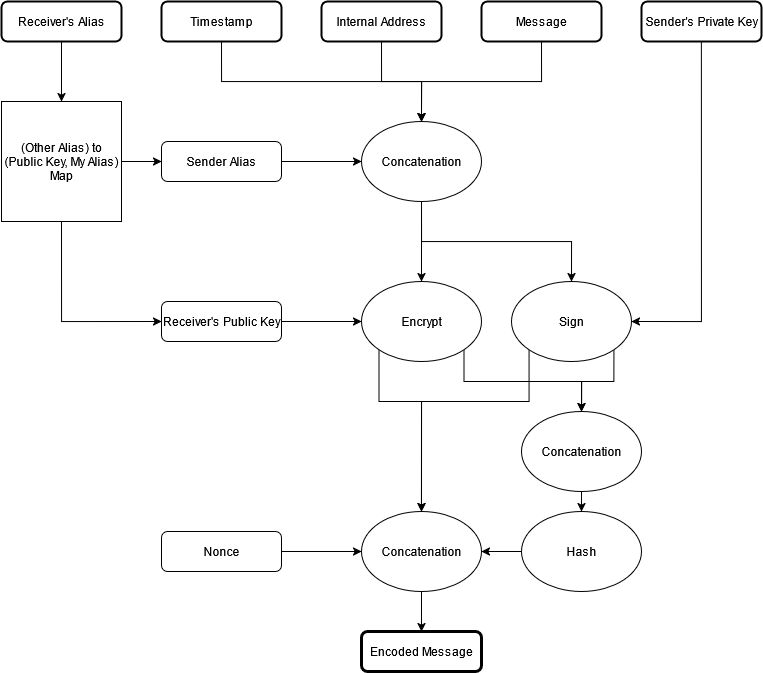
\includegraphics[width=0.55\linewidth]{encode_nbg.png}
    \caption{Message encoding process}
\end{figure}

Hash: It is used to determine whether the relaying nodes have already seen this message. It prevents infinite looping relays. A proof-of-work (PoW) requirement must be met to minimize spam and tampering similar to Bitcoin \cite{bitcoin2008}. 
However, the nonce is excluded from the hash calculation.
PoW difficulty is chosen to cap the global theoretical message rate, ensuring that even high-performance nodes cannot flood the network beyond a theoretical maximum. This cost is incurred only by the sender, making it a user-side performance trade-off.\\
Encryption: The encryption allows only the intended receiver to view the message and also metadata such as sender alias, internal address, and timestamp.\\
Signature: The receiver verifies the message integrity and authenticity using the sender’s public key and signature. Inclusion of the timestamp in the signature serves as a simple counter to general replay attacks.


\section{Decoding and Relaying}

\texttt{Timestamp of reception}: The timestamp of data reception is recorded.\\
\texttt{Deduplication}: The hash and nonce are extracted. Hash validity and the PoW is then verified. Every node keeps a record of hashes of previously relayed messages. If it has seen the hash, the message is discarded. If not, the hash is added to the record and the message is relayed to all neighbors.\\
\texttt{Decryption}: The node then attempts decryption on the encrypted part. If decryption fails, the message is discarded. Otherwise, the original components are extracted (timestamp of creation, sender alias, internal address, and decoded message).\\
\texttt{Verification}: The node then looks up the sender’s public key using the sender alias. If the alias is not found, the message is treated as \texttt{anonymous}, and the signature is not verified. Otherwise, the decryption product is used to verify the signature using the sender’s public key.\\
\texttt{Aging}: The node verifies that the age of the message (difference between current timestamp and timestamp of creation) is less than the maximum message age. The maximum message age depends on how long the hash is stored by the node and can be different for different nodes.\\
\texttt{Result}: The decoded message data, timestamp of reception, timestamp of creation, sender alias, and internal address are the result of decoding.

\begin{figure}[h]
    \centering
    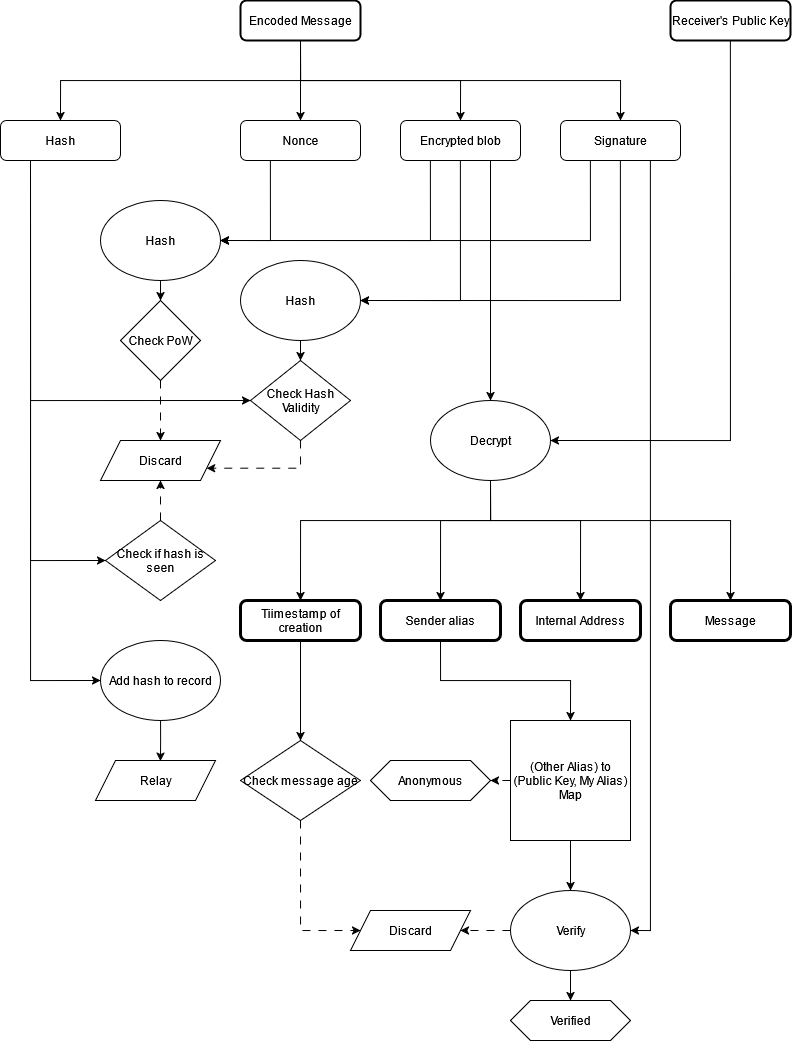
\includegraphics[width=0.55\linewidth]{decode_nbg.png}
    \caption{Message decoding and relay process}
\end{figure}

\section{Optional Improvements}
\texttt{Sector-based routing}: To improve efficiency in large networks, the message can be flooded in only specific regions called \texttt{sectors}, which is an arbitrary group of nodes. However, this may come at the cost of a greater risk of deanonymization of the receiver and sender. Moreover, the sender must know in which sector the receiver is in.\\
\texttt{Time To Live}: TTL is used in structured systems, but here topologies are unknown and dynamic. It may also increase the risk of deanonymization. It could be used for niche cases.\\
\texttt{Better Seen-Hash}: The record of hashes of previously relayed messages can grow uncontrollably. It may be cleared after a random time or after reaching a size limit. Bloom filters or other data structures may be used.\\
\texttt{Periodic key rotation}: Compromising a private key compromises all past messages encrypted to that key. Ephemeral keys or periodic key rotation may be used.\\
\texttt{Dummy traffic}: Attempts of traffic analysis can be nullified by nodes creating and relaying dummy messages and/or relaying messages only after a short duration of random time.\\
\texttt{Replay Attacks}: Replay is prevented via deduplication using PoW hash, signatures, and aging rules on relaying nodes. A replay will result in an immediate message drop by the attacker's neighbors since the hash is already seen, and by the receiver if the age is exceeded. More rules can be implemented on top, including session or one-time tokens or message counters.\\
\texttt{HMAC-based Signatures}: Instead of public-key signatures, implementations can optionally use keyed HMAC signatures for message integrity verification. This improves performance but requires a pre-shared per-sender secret between sender and receiver at bootstrap.\\
\texttt{Alternative Proof-of-Work Mechanisms}: Standard proof-of-work is vulnerable to adversaries with high-end parallel hardware (GPUs, ASICs). A better alternative is the use of Verifiable Delay Functions (VDFs) \cite{vdf2019}. VDFs require a specific duration of sequential computation, effectively neutralizing the advantage of parallel processors. This also providing more predictable message verification times.\\
\texttt{Tagged Decryption}: A short, non-secret tag can be prepended to the encrypted blob to indicate the intended receiver. Nodes can quickly check this tag before attempting decryption. However, this may also increase the risk of deanonymization.\\

EFPIX deliberately prioritizes maximum anonymity and resilience over performance (“0\% performance, 100\% security” by default). Optional optimizations such as sector-based routing or TTL may increase scalability but reduce anonymity. The choice depends entirely on application requirements.

\section{Example Instantiation}
EFPIX defines the protocol framework, flow, and components conceptually. The exact format, contents, cryptographic specifics, etc., are left to implementations. Implementations must tune PoW, hash memory limits, and safe key management to achieve optimal performance and security.
However, an example instantiation is provided here. Implementations may use larger key sizes to increase the payload fraction (at the cost of slower cryptographic operations) or omit signatures for single-use anonymous messages to further reduce overhead.\\

This example uses RSA 2048 \cite{rsa1978} with 11 bytes OAEP padding \cite{oaep1995}, SHA-512 hash \cite{sha512} and 2 leading zeros for the PoW. This example uses RSA for simplicity. However, a production-grade implementation should consider elliptic-curve cryptography (ECC) or post-quantum public-key encryption for improved efficiency and long-term security. \\

Pre-encryption data format (245 bytes)
\begin{table}[h]
\centering
\begin{tabular}{|c|c|c|c|}
\hline
\textbf{Timestamp} & \textbf{Sender Alias} & \textbf{Internal Address} & \textbf{Message} \\
\hline
9 bytes & 16 bytes & 4 bytes & Up to encryption limit 216 bytes \\
\hline
\end{tabular}
\end{table}

Encoded message layout (580 bytes)
\begin{table}[h]
\centering
\begin{tabular}{|c|c|c|c|c|}
\hline
\textbf{Version} & \textbf{Hash} & \textbf{Nonce} & \textbf{Encrypted blob} & \textbf{Signature} \\
\hline
1 bytes & 64 bytes & 3 bytes & 256 bytes & 256 bytes \\
\hline
\end{tabular}
\end{table}

The protocol allows for extensibility. Optional headers can be used for the improvements based on the version byte, which enables future format upgrades. 

\section{Threat Model and Security Analysis}

\subsection{Adversary Model}

\texttt{Passive Eavesdropper}: Observes network traffic without modifying it.\\
\texttt{Active Adversary}: Can inject, modify, or replay messages. May act as a participating node.\\
\texttt{Compromised Node}: A legitimate node acting maliciously, leaking keys or dropping messages.\\
\texttt{Global Passive Observer (GPO)}: Observes all network traffic, attempting to correlate timing or metadata.\\
\texttt{Circling Adversary}: Controls a majority of surrounding nodes to localize message origin.\\
\texttt{Sybil Attacker}: Launches many fake nodes to gain influence or disrupt hashing and routing.\\
\texttt{Replay Attacker}: Re-broadcasts valid messages to cause confusion or traffic analysis.

\subsection{Security Properties}

\texttt{Passive Eavesdropping}: Encryption hides message content and metadata, as encrypted blob is opaque to observers. \\
\texttt{Active Modification}: Messages are protected by digital signatures and hash verification. Tampered messages are discarded. \\
\texttt{Compromised Nodes}: Flooding ensures alternate paths unless a compromised node becomes a topological choke point. \\
\texttt{Sybil \& Global Observation \& Circling Attack}: EFPIX does not claim to solve this problem, as it is an inherent trade-off for achieving a decentralized, topology-agnostic, and server-less design. Implementations may add random delays before relaying to mitigate, but not eliminate, this risk. \\
\texttt{Denial of Service}: While PoW and VDFs impose a significant cost on message creation, a sufficiently resourced adversary might be able to degrade the network's performance by flooding it with valid messages. The protocol aims to make such attacks economically expensive, but does not claim to make them impossible.\\
\texttt{Replay Attack}: Timestamps in signatures, PoW hash, and age rules prevent simple replays; message counters and tokens can be used on top.

\subsection{Comparison with Related Protocols}

\begin{table}[h]
\centering
\begin{tabular}{|c|c|c|c|c|}
\hline
\textbf{Feature} & \textbf{EFPIX} & \textbf{Tor \cite{tor2004}} & \textbf{Bitmessage \cite{bitmessage2012}} & \textbf{Matrix \cite{matrix2014}} \\
\hline
Topology-agnostic      & \cmark & \xmark & \cmark & \xmark \\
End-to-End Encryption  & \cmark & \cmark & \cmark & \cmark \\
Metadata Protection    & \cmark & Partial & Partial & \xmark \\
Anonymity              & Probabilistic & Strong & Moderate & \xmark \\
Sybil Resistance       & Partial & \xmark & \xmark & \xmark \\
Offline Messaging      & \cmark & \xmark & \cmark & \cmark \\
Broadcast Suitability  & \cmark & \xmark & \cmark & \xmark \\
GPO Resistance         & Partial & \xmark & \xmark & \xmark \\
\hline
\end{tabular}
\caption{Comparison of EFPIX with selected secure communication protocols}
\end{table}

\section{Future Work}
Future work could explore efficient and secure partial flooding strategies, integration with radio mesh hardware, and secure bootstrap methods for alias public key exchanges. Implementations can simulate or deploy on different networks to provide performance and other results to compare against existing protocols that aim to solve a similar problem. 

\section{Conclusion}
EFPIX provides a robust framework for secure and censorship-resistant communication, protecting against invasive and potentially malicious surveillance. It also conceals “non-content” data from prying eyes. Its decentralized, flooding-based design ensures delivery even in restricted or faulty environments, making it an ideal option for disconnected, totalitarian, or disaster-struck areas.

\begin{thebibliography}{10}
\bibitem{bamford2012}
J. Bamford, \textit{The NSA Is Building the Country’s Biggest Spy Center (Watch What You Say)}, 
\url{https://www.wired.com/2012/03/ff-nsadatacenter}, 2012.

\bibitem{heilman2014}
E. Heilman, \textit{A Brief History of NSA Backdoors}, 
\url{https://ethanheilman.tumblr.com/post/70646748808/a-brief-history-of-nsa-backdoors}, 2014.

\bibitem{pegasus2023}
European Parliament, \textit{Investigation of the use of Pegasus and
equivalent surveillance spyware}, 
\url{https://www.europarl.europa.eu/RegData/etudes/ATAG/2023/747923/EPRS_ATA(2023)747923_EN.pdf}, 2023.

\bibitem{snowden2014}
\textit{Edward Snowden: Leaks that exposed US spy programme}, 
\url{https://www.bbc.com/news/world-us-canada-23123964}, 2014.

\bibitem{apple2025}
\textit{Apple pulls data protection tool after UK government security row}, 
\url{https://www.bbc.com/news/articles/cgj54eq4vejo}, 2025.

\bibitem{bitcoin2008}
S. Nakamoto, \textit{Bitcoin: A Peer-to-Peer Electronic Cash System},  \url{https://bitcoin.org/bitcoin.pdf}, 2008.

\bibitem{vdf2019}
Dan Boneh, Joseph Bonneau, Benedikt Bunz, and Ben Fisch, \textit{Verifiable Delay Functions},  
\url{https://eprint.iacr.org/2018/601.pdf}, 2019.

\bibitem{rsa1978}
R. L. Rivest, A. Shamir, and L. Adleman, \textit{A Method for Obtaining Digital Signatures and Public-Key Cryptosystems},  
\url{https://people.csail.mit.edu/rivest/Rsapaper.pdf}, 1978.

\bibitem{oaep1995}
Mihir Bellare, Phillip Rogaway, \textit{Optimal Asymmetric Encryption - How to Encrypt with RSA},  
\url{https://cseweb.ucsd.edu/~mihir/papers/oaep.pdf}, 1995.

\bibitem{sha512}
National Institute of Standards and Technology (NIST), \textit{FIPS PUB 180-4: Secure Hash Standard (SHS)}, 
\url{https://nvlpubs.nist.gov/nistpubs/FIPS/NIST.FIPS.180-4.pdf}, 2015.

\bibitem{tor2004}
R. Dingledine, N. Mathewson, and P. Syverson, \textit{Tor: The Second-Generation Onion Router}, \url{https://www.usenix.org/events/sec04/tech/dingledine.html}, 2004.

\bibitem{bitmessage2012}
J. Warren, \textit{Bitmessage: A Peer-to-Peer Message Authentication and Delivery System} \url{https://bitmessage.org/bitmessage.pdf}, 2012.

\bibitem{matrix2014}
M. Hodgson and A. Le-Prevost, \textit{Matrix: An Open Network for Secure, Decentralized Communication} \url{https://matrix.org/docs/spec}, 2014.

\end{thebibliography}

\end{document}
